\newpage
\chapter{Umsetzung}

\section{Struktur}
Um die Messages sowohl auf dem Server als auch auf dem Android App verfügbar zu machen, wurden diese in ein seperates Projekt ausgelagert. Weiter wurde festgestellt, dass gewisse Sachen auf beiden System genutzt werden muss, daher wurde die gesammte Serialisierungs und Deserialisierungskomponente in das Commons Projekt ausgelagert. Es wird jeweils nach MavenLocal deployed um es in den anderen Projekten verfügbar zu machen.


\section{Verwendete Bibliotheken}
\subsection{Commons}
\begin{tabularx}{\textwidth}{|X|X|c|X|}
	\hline
	\textbf{Name} & \textbf{Verwendungszweck} & \textbf{Version} & \textbf{Lizenz} \\
	\hline \hline
	Google GSON & Java Serialisierungs / Deserialisierungs Bibliothek & 2.6.2 & Apache 2.0\\
	\hline 
\end{tabularx}


\subsection{Server}
\begin{tabularx}{\textwidth}{|X|X|c|X|}
	\hline
	\textbf{Name} & \textbf{Verwendungszweck} & \textbf{Version} & \textbf{Lizenz} \\
	\hline \hline
	Hibernate ORM Mapper & Objekt-Relationales mapping zwischen Datenbank und Models  & 5.1.0 & Apache 2.0\\
	\hline 
	RabbitMQ Client & Client Komponente zur Kommunikation mit dem Rabbit MQ Server & 3.6.0 &  Mozilla Public License 1.1, GPL 2, Apache 2.0 \\
	\hline 
	jGraphT & Graph Bibliothek für Java, um effizient Operationen auf dem Graph auszuführen & 0.9.2 &  LGPL, EPL \\
	\hline 
\end{tabularx}

\subsection{Onboard App}
\begin{tabularx}{\textwidth}{|X|X|c|X|}
	\hline
	\textbf{Name} & \textbf{Verwendungszweck} & \textbf{Version} & \textbf{Lizenz} \\
	\hline \hline
	DroneKit-Android Client & Android API für MAV-Link Protokoll zum ansteuern der Drohne & 1.5.1 & Apache 2.0\\
	\hline 
	AMQP Messaging Library & Messaging für Android & 3.6.0 &  Mozilla Public License 1.1, GPL 2,  Apache 2.0 \\
	\hline 
	Lyra  & High availability Messaging & 0.4.3 &  Apache 2.0 \\
	\hline 
\end{tabularx}
\subsection{Customer App}
\begin{tabularx}{\textwidth}{|X|X|c|X|}
	\hline
	\textbf{Name} & \textbf{Verwendungszweck} & \textbf{Version} & \textbf{Lizenz} \\
	\hline \hline
	Paypal Forms & Paypal integration für Xamarin.Forms & 2.0.4 & MIT \\
	\hline 
	Xamarin Forms & Messaging für Android & 2.2.0.45 & \url{https://www.xamarin.com/license} \\
	\hline 
\end{tabularx}


\section{Implementierung}

\subsection{Code Standard}
Im Team wurden folgende Code-Conventions eingeführt.

\subsubsection{Autorfreie Klassen}
In Java wird klassicherweise der Autor im Javadoc Kommentar in der Klasse angegeben.

\begin{lstlisting}
/**
 * @author Kirusanth Poopalasingam (pkirusanth@gmail.com)
 */
public class MyTestClass{
}
\end{lstlisting}
Der Autor in der Klasse suggeriert, dass nur ein Autor für diese Klasse existiert und für diese Klasse verantwortlich ist. Dies sollte aber nicht der fall sein, da jedes Teammitglied verantwortlich für die gesammte Code-Qualität ist und zudem ist die Angabe auf der Klasse heutzutage mit einem Version Control System redundant.

\subsubsection{Javadoc}
Generell sollte Javadoc nur dort verwendet werden, wo es nötig ist. Da es sich bei Projekt Helin nicht um eine API handelt, sollten auch die Methoden und Parameter nicht redundant dokumentiert werden. Ein Beispiel für eine schlechte Javadoc Dokumentation sieht folgendermassen aus:
\begin{lstlisting}
// Beispiel einer Play Klasse
public final class ConfigUtil {
    private ConfigUtil() { }

    /**
     * Quotes and escapes a string, as in the JSON specification.
     *
     * @param s
     *            a string
     * @return the string quoted and escaped
     */
    public static String quoteString(String s) {
        return ConfigImplUtil.renderJsonString(s);
    }
    // ...
}
\end{lstlisting}
Bei der Methode quoteString() kann der ganze Javadoc Kommentar weggelassen werden, da er nicht mehr Aussagekraft hat, als die Methode selbst. Stattdessen sollte die Methode so geschreiben werden, dass die Namen aussagekräftiger sind.
\\
Eine bessere Implementierung würde folgendermassen aussehen:
\begin{lstlisting}
public final class ConfigUtil {
    private ConfigUtil() { }

    public static String quoteStringAccordingToJsonSpecification(String unquotedJson) {
        return ConfigImplUtil.renderJsonString(unquotedJson);
    }
    // ...
}
\end{lstlisting}
\subsubsection{Code}
Für die Formatierung und den Static Check werden die 'Code Inspection' von IntelliJ IDEA verwendet.
\\
Es handelt sich bei den 'Code Inspections' um konfigurierbare Regeln, welche mit dem Projekt in das Repository eingecheckt werden. Die Entwicklungsumgebung führt die 'Code Inspections' vor dem Einchecken aus und weisst gegebenenfals auf Unstimmigkeiten hin.
Da sich die standard Regeln von IntelliJ bereits in anderen Projekten bewährt haben, wurde von einem eigenen Standart abgesehen.
\newpage
\subsection{Messaging}
Um die nichtfunktionalen Anforderungen im Bereich der Kommunikation zu erfüllen, wurde AMQP als Protokoll ausgewählt. Mit Messaging soll gewährleistet werden, dass die Verbindungswiederherstellung funktioniert. Die funktionale Anforderung des Missionsabbruchs wird somit soweit gedeckt, dass versucht wird die Verbindung aufrechtzuerhalten, sofern das Netz es erlaubt. Bei kurzen Netzunterbrüchen kann somit über das AMQP Protokoll eine Verbindung zur Drohne gewährleistet werden.

\begin{itemize}
	\item{\textbf{Verbindungsabbruch:} \\
	Gemäss den nicht funktionalen Anforderungen darf der Verbindungsabbruch keinen Einfluss auf die Mission haben. Um gemäss den funktionalen Anforderungen einen Missionsabbruch zu gewährleisten, wird versucht Unterbrüche so kurz wie möglich zu halten und einen automatischen Verbiundungsaufbau zu ermöglichen. Aus diesem Faktoren wird die gesamte Mission vor dem Start übertragen, damit sie ausgeführt werden kann. Einzelne Wegpunke sind somit nicht auf eine stabile Internetverbindung angewiesen, da die Route bereits von Anfang bekannt ist. Der Missionsabbruch ist ebenfalls gewährleistet - sofern die GSM Verbindung besteht. 
	\\
	Verbindungsabbrüche auf dem Mobiltelefon haben zweierlei Konsequenzen:	
	\begin{itemize}
		\item{\textbf{Mobiltelefon kann die Messages vom Server nicht empfangen:} \\
		Dieses Szenario wird durch das RabbitMQ abgefangen. Der Messaging Broker cached die Nachrichten solange bis der Consumer (Mobiltelefon) wieder verfügbar ist. Es besteht somit kein zusätzlicher Handlungsbedarf auf dem Onboard-App.
		}
		\item{\textbf{Messages vom Mobiltelefon zum Server können nicht gesendet werden:} \\
		In diesem Fall kann der Übertragungsfehler nicht durch RabbitMQ abgefangen werden. Der Broker hat vom Producer (Mobiletelefon) noch keine Nachricht bekommen. Aus diesem Grund wird producerseitig eine Exception geworfen, die darauf hinweist, dass die Verbindung unterbrochen ist. In diesem Fall wird die Nachricht in einem Queue zwischengespeichert. Sämtliche Folgenachrichten, die während des Verbindungsunterbruchs nicht übertragen werden können, werden ebenfalls in dieser Queue gespeichert. Sobald die Verbindung wieder besteht, werden die Nachrichten aus der Queue gesendet.
		}
	\end{itemize}
	Mit diesen Massnahmen ist ein guter Kompromiss aus Zuverlässigkeit und Aufwand entstanden. Alle missionskritischen Nachrichten können übertragen werden. Telemetriedaten sind von einem Verbindungsausfall ebenfalls nicht betroffen.
	}
	\item{\textbf{Verbindungswiederherstellung:}
	Aus den nicht funktionalen Anforderungen ist zu entnehmen, dass bei einem Verbindungsunterbruch ein Reconnect statt findet. Dieser Reconnect soll, sobald die Verbindung im GSM Netz wieder besteht nicht länger als 30s dauern. \\
	Bei der Konfiguration von AMQP bestanden mehrere Möglichkeiten. Einersetis war der bekannte Backoff Algorithmus eine Option. Dieser Algorithmus arbeitet nach einem incrementellen Prinzip. Je länger der Unterbruch dauert, desto länger dauert es bis er die Verbindung wieder versucht aufzubauen. Auf der anderen Seite stand ein einfacher Interval-Algorithmus. Dieser versucht alle drei Sekunden die Verbindung wiederherzustellen, bis zum erfolgreichen Verbindungsaufbau. Mit diesen Erkenntnissen haben wir folgende Messung gemacht:
	\begin{center}
		\begin{tabular}{|r|r|}
		\hline
		  \textbf{Backoff} & \textbf{Interval 3s} \\
		\hline
		  17 & 7 \\
		  7 & 7 \\
		  9 & 7 \\
		  11 & 7 \\
		  10 & 7 \\
		\hline
		% TODO: Kommentar noch: Anzahl Sekunden bis zum Verbindungsaufbau
		\end{tabular}
	\end{center}
	Aus diesen Erkenntnissen standen beide Möglichkeiten offen, denn beide erfüllen die Anforderungen und haben somit auch keine Auswirkungen auf die Qualität. Am Ende wurde bewusst auf den BackOff Algorithmus gesetzt. Der Backoff Algorithmus benötigt zwar deutlich länger für einen Reconnect als das fixe Zeitinterval. Die hetrogene Verteilung der Wiederverbindungszeiten spricht aber für den Backoff Algorithmus. Sollte es zu Probleme auf der Serverseite kommen, so werden nicht alle Geräte gleichzeitig einen Reconnect probieren - der Reconnect passiert somit gestaffelt. Dies bringt zusätzlich Stabilität ins System.}
	\item{\textbf{Android Process Lifecycle:} \\
	Da die OnboardApp auf einem Android Betriebssystem läuft, mussten gewisse Voraussetzungen geprüft werden. Im Grund kann davon ausgegangen werden, dass die Applikation immer im Vordergrund steht. Es ist doch sehr unwahrscheinlich, dass die Appliaktion in den Hintergrund rückt, weil eine andere Applikation verwendet wird. \\
	Laut Android Dokumentation ist das Verhalten einer Applikation im Hintergrund nicht deterministisch \cite{androidGuide}. Sollte eine Applikation im Hintergrund gewisse Garantien haben, so muss von einem Service und der spezifischen Implementierung eines Services gesprochen werden. Im Fall der OnboardApp und den getroffenen Annahmen, wurde davon abgesehen, da die Applikation während des Fluges nicht gewechselt wird.
	}
\newpage
\end{itemize}

\section{Customer App}
Gemäss Aufgabenstellung sollte ein "'Prototyp einer Android App"', mit welchen Bestellungen am System abgegeben können, entwickelt werden.
Dieser App wurde bewusst als letzte Komponente entwickelt, denn es wurde zuerst geschaut, dass die Server und On-Board Komponente reif genug waren.

Um nicht auf die Funktionalität der Customer-App zu verzichten, wurden in der Administrator-Seite eine "'Fake Order"' Funktionen eingeführt. 
Diese imitiert dem Bestellprozess des Kunden uns schickt eine Anfrage mit vordefinierten Koordinaten und Produkten an das System. 
Dies war für den Anfang der Entwicklung Ausreichend war. Doch schnell kamen Limitierung dieser Möglichkeit. Denn beim Testen war es wichtig mit unterschiedlichen Projekten und Positionen zu testen. 
\begin{figure}[h]
	\centering
	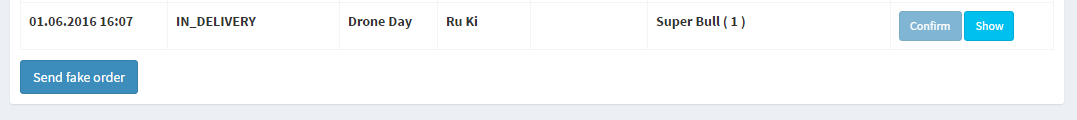
\includegraphics[width=1\textwidth] {images/customer-app-fake-order.png}
	\caption{Send Fake Order within Administrator Page}
\end{figure}
Daher wurde die Customer-App, mit dem Fokus die Fake-Order-Funktion abzulösen, entwickelt.
Entgegen dem On-Board-App, welches mit mit Java nur für Android entwickelt wurden, für das Customer-App auf Xamarin Forms gesetzt.
Auch wenn gemäss der Aufgabenstellung ein Android App gengüt hätte, war doch die Fragen offen, wie die iPhone Kunden ein Bestellung tätigen können.
Mit einem Marktanteil von 42.2\% (Zahlen 2015) \cite{ios-user} von iOs Benutzern in der Schweiz, ist anzunehmen dass die Anforderung nach einem iPhone App kommen wird.
Deshalb wurde, nach Absprache mit dem Betreuer, auf C# und Xamarin Forms gesetzt, so kann auch gleichzeitig eine iOS App entwickelt werden - ohne grossen Aufwand.

\subsection{Resultate}
\begin{landscape}
\begin{figure}[h]
	\centering
	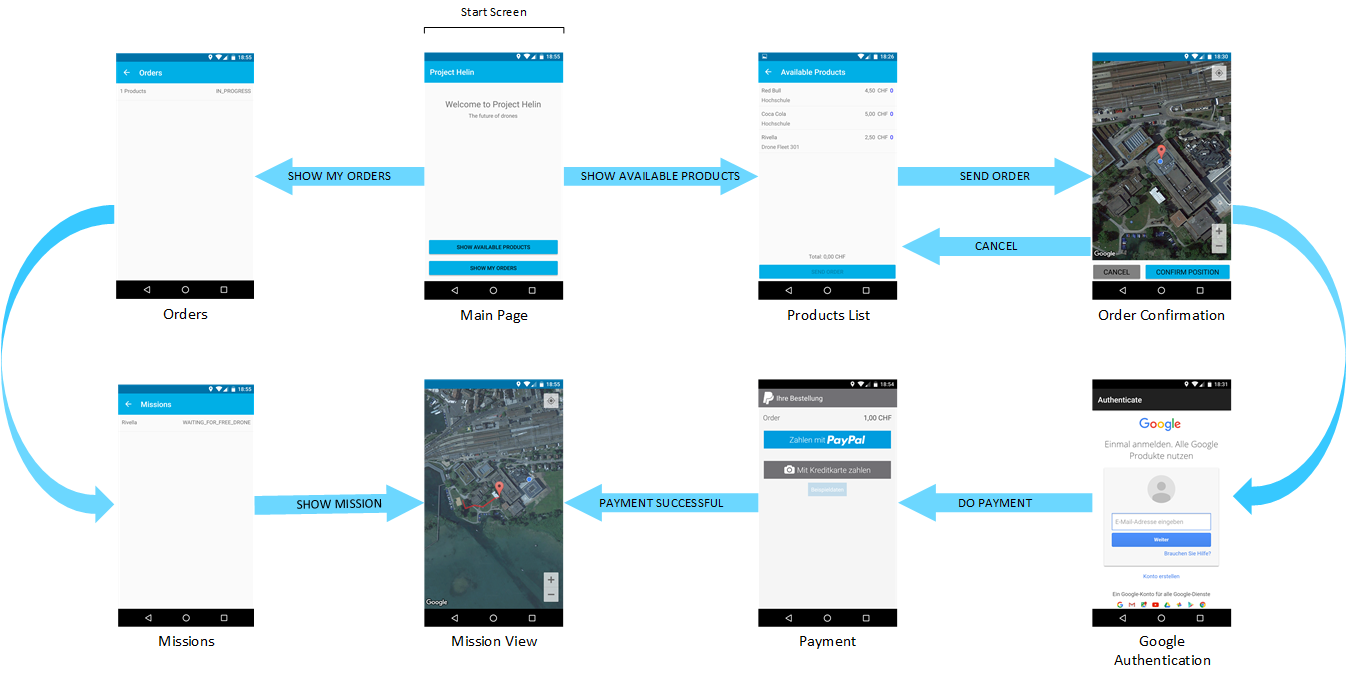
\includegraphics[width=0.8\paperheight] {images/customer-app-pages.png}
	\caption{Customer app flow}
\end{figure}
\end{landscape}

Die App wurde bewusst einfach gehalten.
Auf dem Start Screen kann der Kunde auswählen, ob er seine alten Bestellungen sehen oder neue Produkte bestllen will.
Beim Bestellen neuer Produkte, werden alle aufgelistet, welche sich innerhalb der Bestellezone liegen.
Nach dem Abschicken der Bestellung, bekommt der Kunde einen Vorschlag für die Abwurfsposition.
Falls er sich überlegt, doch nicht zu bestellen, springt er wieder zurück auf die Produkteliste.
Bis zum letzten Schritt war keine Anmeldung erforderlich.
Im Falle einer Bestätigung der Abwurfsposition, muss sich der Kunde über Google authentizieren lassen.
Danach kann der Benutzer die bestellte Ware bezahlen. Die Bezahlung wird über PayPal abgewickelt.

Nach der erfolgreichen Bezahlung kann wird dem Kunde die Mission angezeigt. 
Der Kunde sieht die Route der Drohne und bei laufend Mission wird die Position der Drohne angezeigt.

